% !TeX root = ../Tex/main.tex

\section{Causal Inference}

\vspace{1em}
The discussion, so far, naturally invites us to make a comparison \textcolor{red}{OR to mirror it} with frameworks that model how hidden factors influence observed outcomes.
Causal inference (\cite{pearlCausalityModelsReasoning2009}) suggests that in order to answer this question we may also think of a "variable" that we are mistakenly excluding from the framework. My guess is that in this context this missing variable exists.

\subsection{Application of Potential Outcome Model}
This section is intended to formalise the intuition thorugh a DAG. Before diving deep into the DAG, I will briefly explain how does the concept of potential outcome applys to this situation, so that non expert readers will \textcolor{red}{comfomfortably go through} the next paragaphs.

\vspace*{1em}
A potential outcome is a counterfactual. Thus, it is a scenario that we do not observe; we think of it as being the closer and most realistic scenario that might have happened in case the actual one didn't.

In the case of the two intaractions I presented, each of them may be considered the counterfactual scenario of the other. Since counterfactuals do not exist, we use real and observed examples to mimic them. The underlieng belief, is that no researcher is as good as reality itself in producing examples of what might have happened. If we trust reality and observation of reality, the role of the researcher is limited to selecting the most appropriate counterfactual from those offered by natural world.

\vspace*{1em}
\textit{Hypothesis:} under no effect of emotions, the case offered by the elephant and the sheperd would have been identical to the one offerd by the other elephant and the tourist.

\subsection{The reason why do I want to use causal inference: from the general case to the single one and back again}
According to \textcite[chap.~2, p.~14]{vonneumannTheoryGamesEconomic1990}: "An almost exact theory of a gas, containing about \(10^{25}\) freely moving particles, is incomparably easier than that of the solar system, made up of 9 major bodies; and still more than that of a multiple star of three or four objects of about the same size. This is, of course, due to the excellent possibility of applying the laws of statistics and probabilities in the first case."

"The problem must be formulated, solved and understood for small numbers of participants before anything can be proved about the changes of its character in any limiting case of large numbers"

In order to follow this suggestion, we go from the general case of the perfect market, and we analyse specific interactions in which that models fails to correctly map reality.

The next step is to use causal inference. Why? because we want again to produce a general case, to pass from the individuality of that interaction to the a \textit{new} general case we need to discard irrelevant differences and variables, and we need to identify a common mechanism. In this way we can produce a new pattern, which will constitute a new map, indeed.

%\subsection{DAGs}
\begin{figure}[htpb] %  figure placement: here, top, bottom, or page
   \centering
   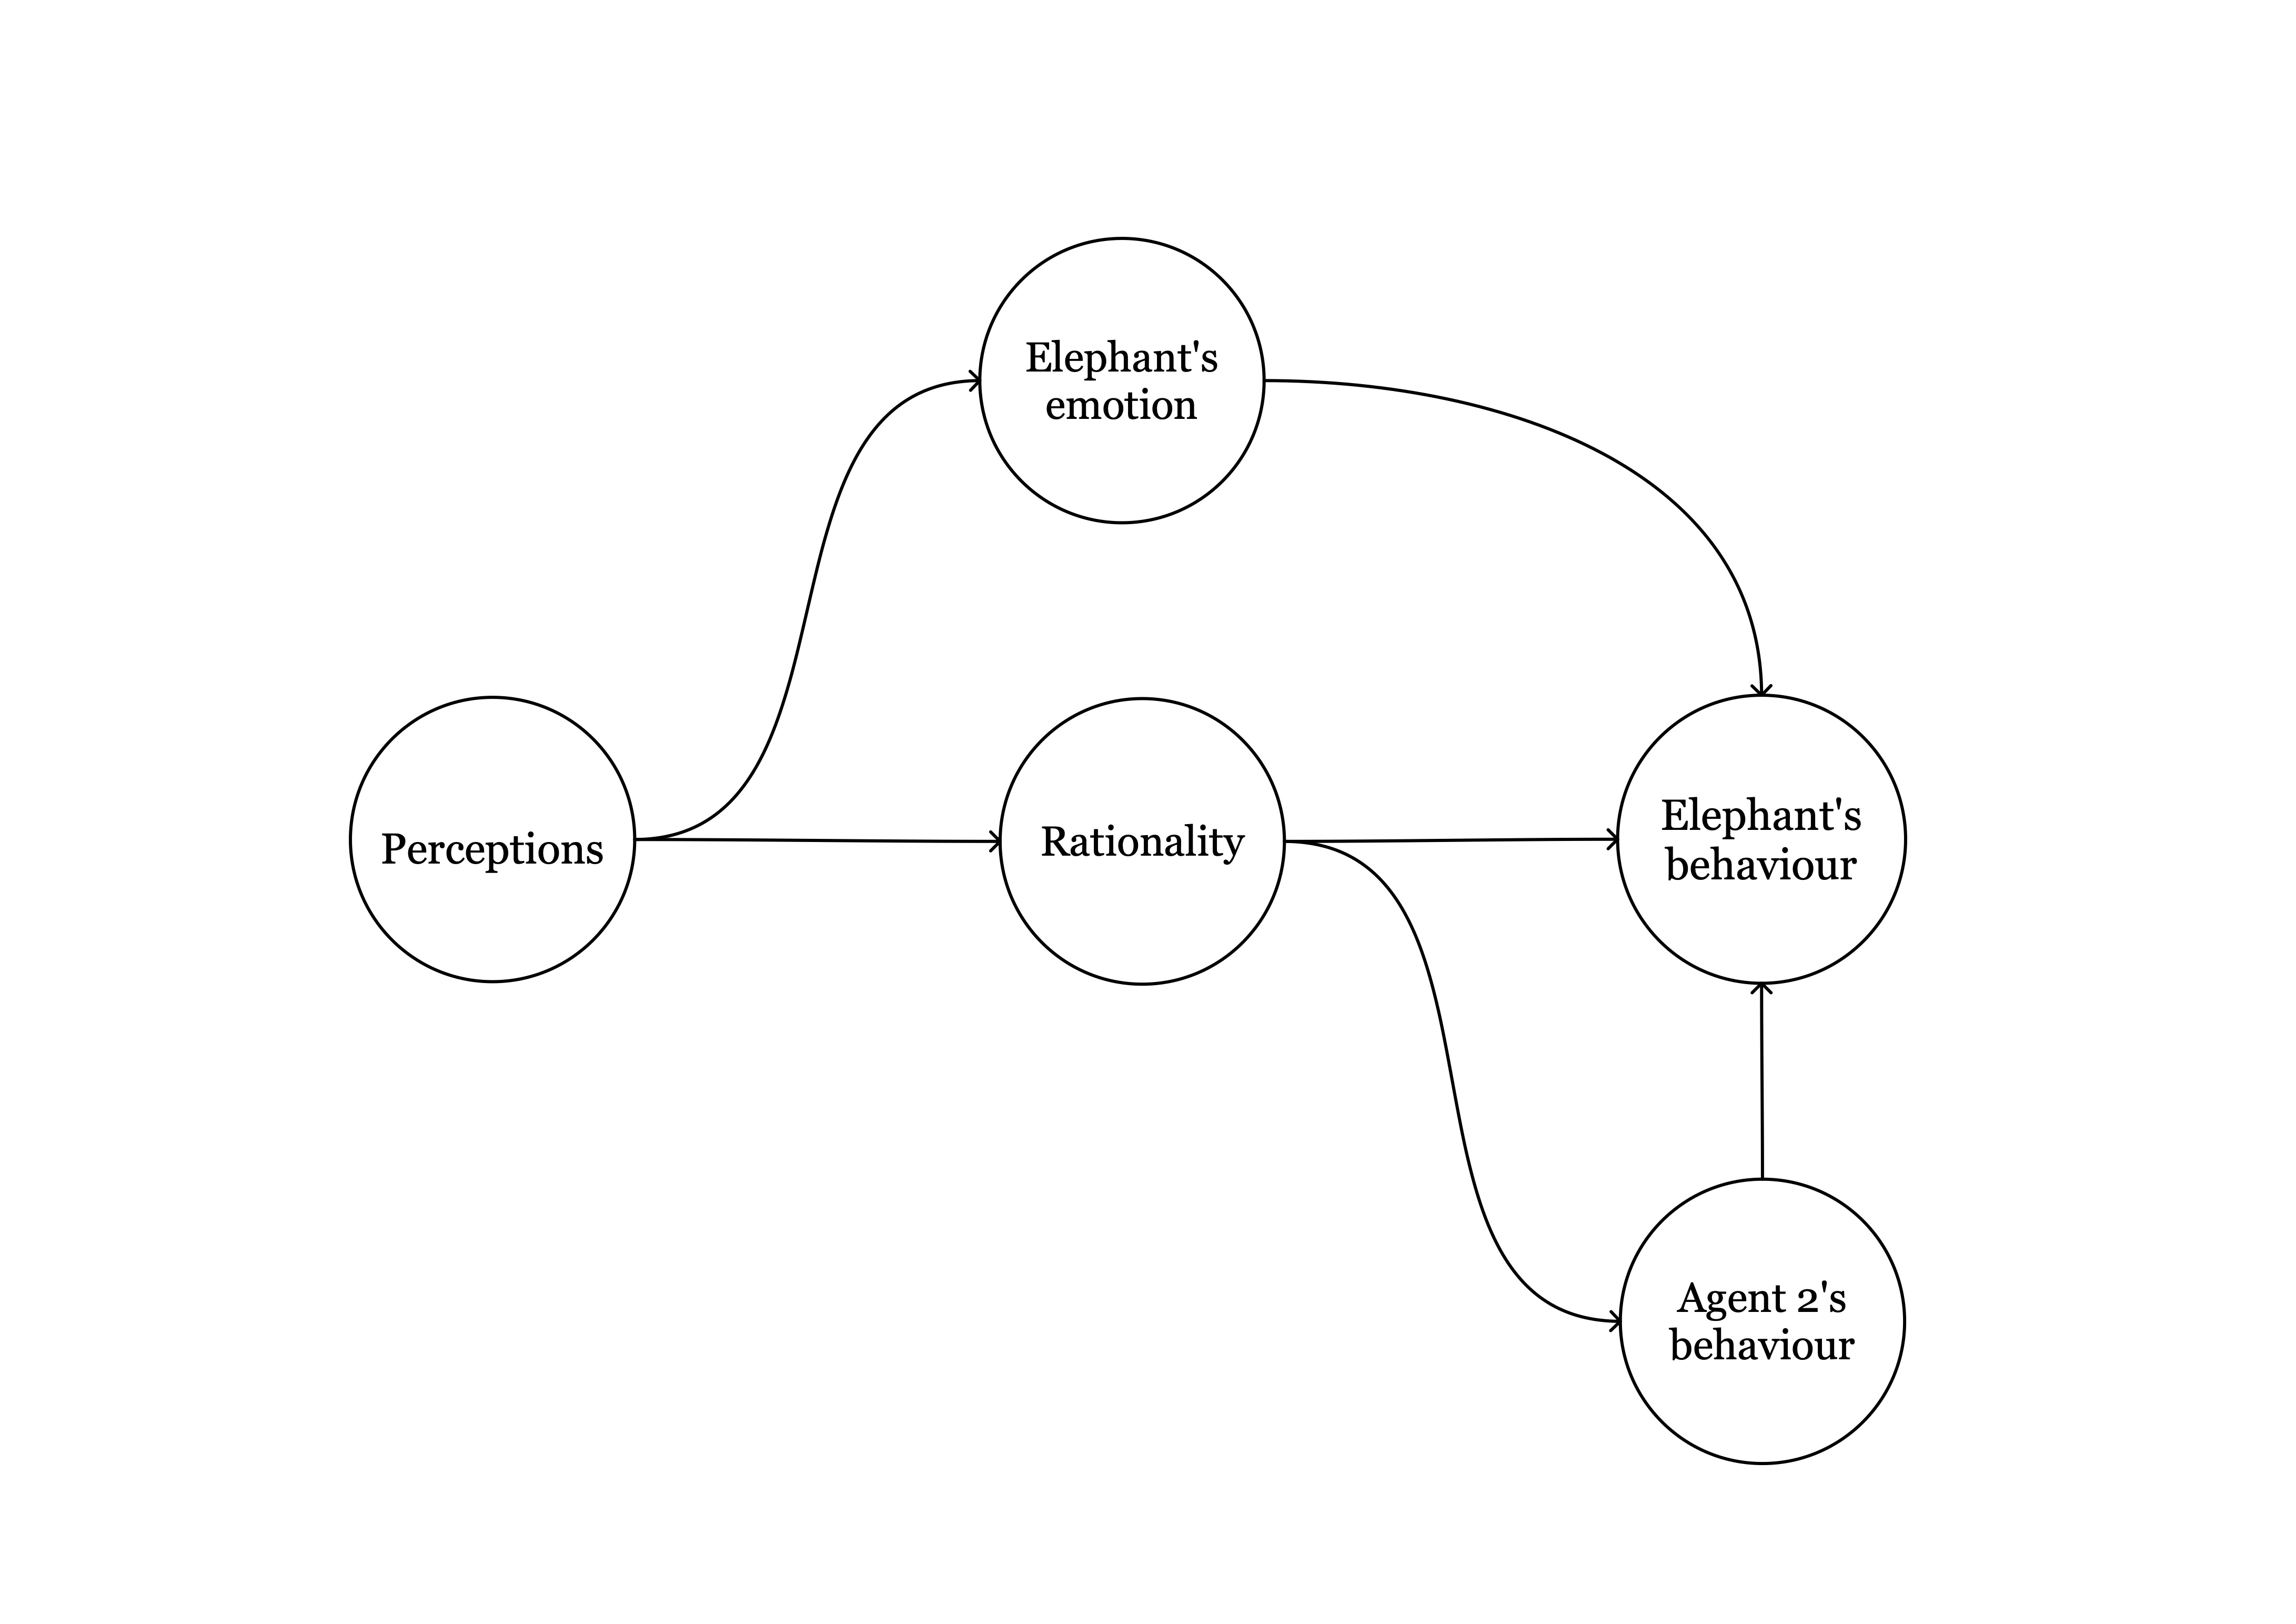
\includegraphics[width=1\linewidth]{Tex/Brauninger.jpg}
  \caption{Un'immagine JPG inclusa in LaTeX.}
  \label{fig:foto}
\end{figure}

